\documentclass[border=10pt]{standalone}

\usepackage{tikz}
\usepackage{tikzsymbols}
\usetikzlibrary{calc,patterns,shapes.geometric}

\def\centerarc[#1](#2)(#3:#4:#5){\draw[#1] ($(#2)+({#5*cos(#3)},{#5*sin(#3)})$) arc (#3:#4:#5);}

\begin{document}
	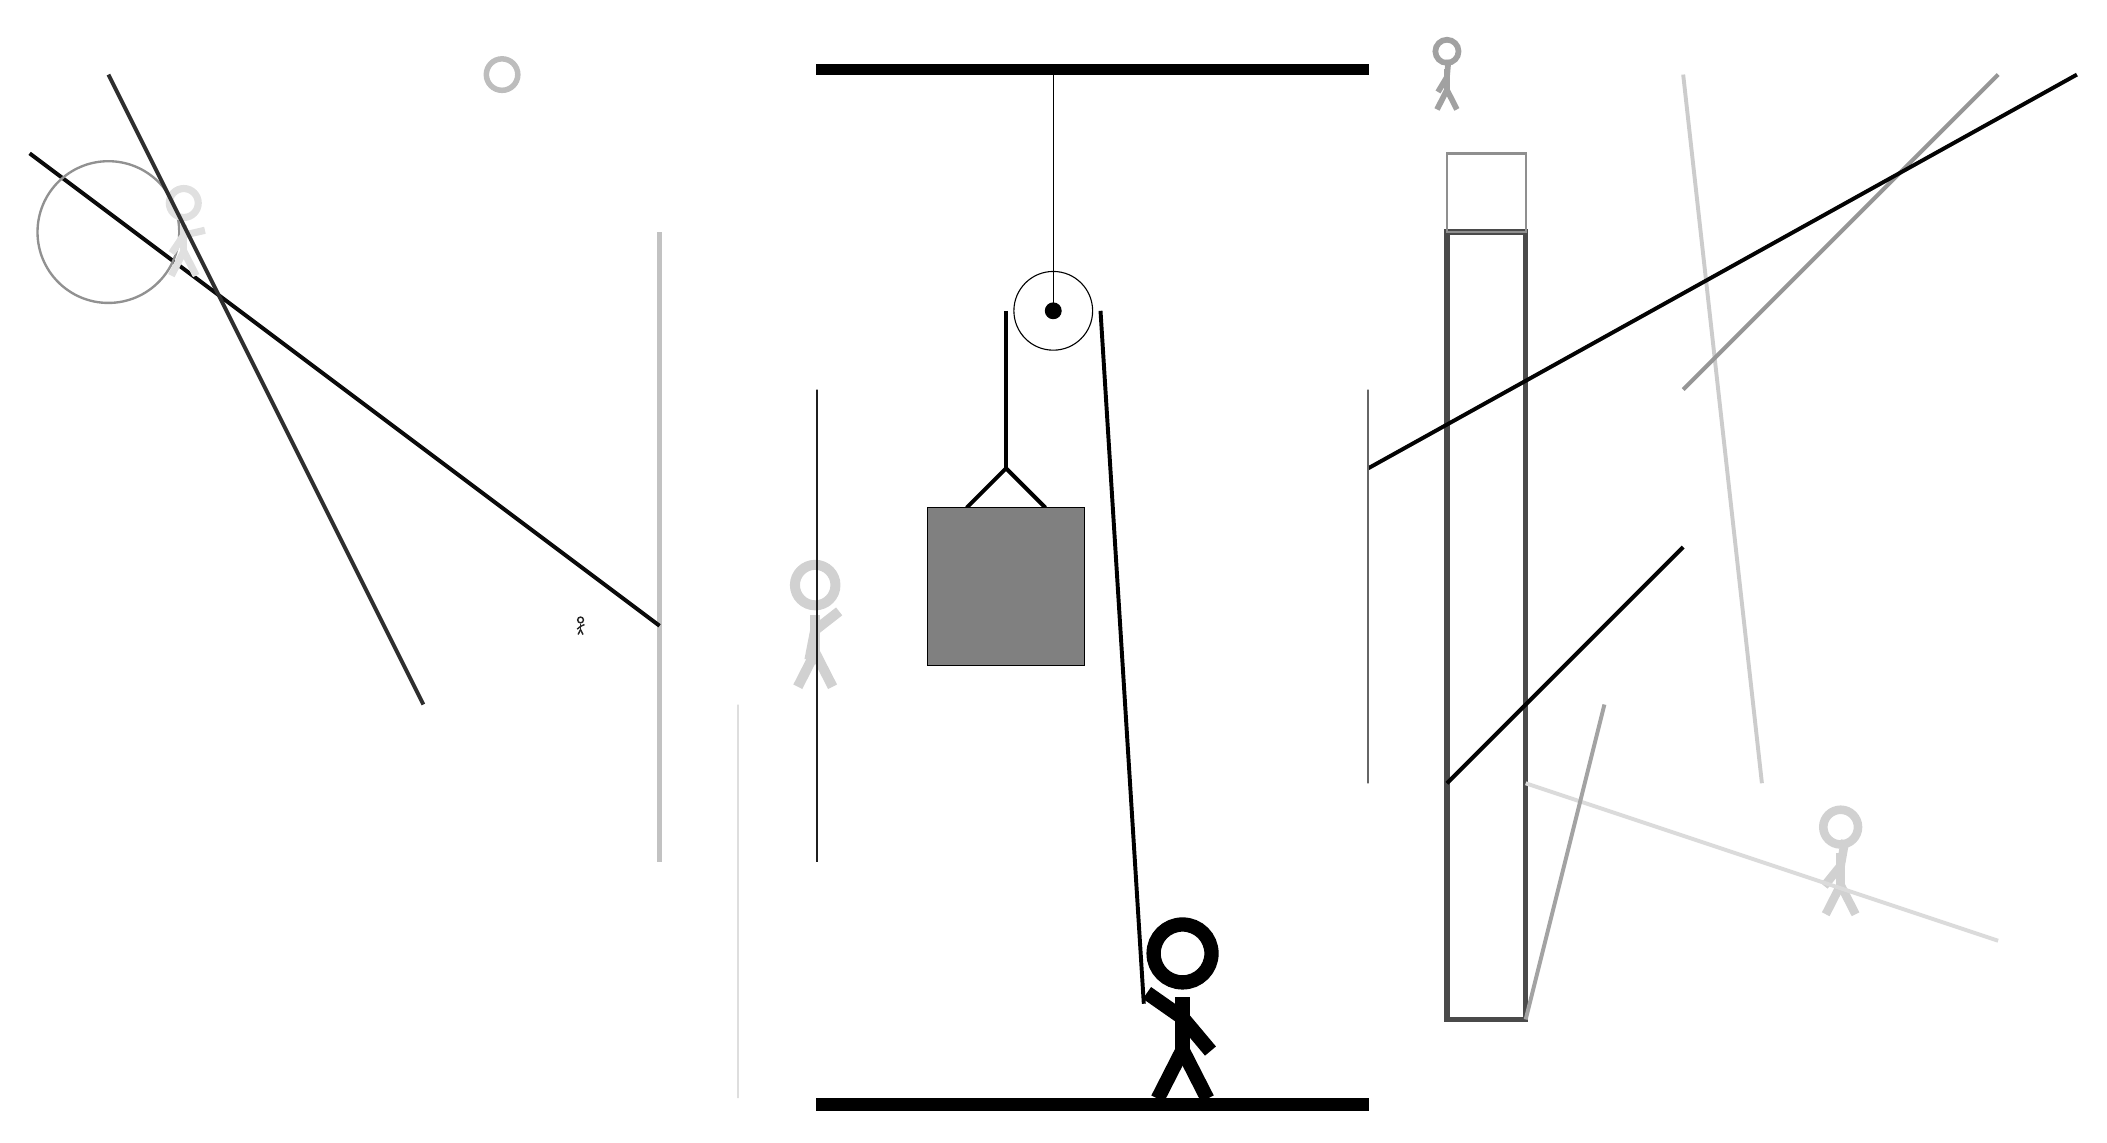
\begin{tikzpicture}
		%%%%% START %%%%%
		
		\draw[fill=black] (-2, 10) rectangle (5, 10.125);
		
		\node[line width=0.7mm, color=black!18] at (-2, 3) {\Strichmaxerl[7][79][38]};
		
		\draw[line width=0.5mm, color=black!20](9, 10) -- (10, 1);
		\node[line width=0.4mm, color=black!18] at (11, 0) {\Strichmaxerl[6][51][80]};
		\draw[line width=0.7mm, color=black!71] (6, -2) rectangle (7, 8);
		
		\draw[line width=0.7mm, color=black!24] (-4, 8) rectangle (-4, 0);
		\draw[line width=0.5mm, color=black!96](-4, 3) -- (-12, 9);
		
		\draw[line width=0.5mm, color=black!41](9, 6) -- (13, 10);
		\draw[line width=0.5mm, color=black!14](7, 1) -- (13, -1);
		\draw[line width=0.5mm, color=black!99](9, 4) -- (6, 1);
		
		\draw[line width=0.3mm, color=black!44] (6, 9) rectangle (7, 8);
		\draw[line width=0.5mm, color=black!99](5, 5) -- (14, 10);
		\draw [line width=0.3mm, color=black!43](-11, 8) circle (0.9);
		\draw[line width=0.5mm, color=black!36](8, 2) -- (7, -2);
		
		\draw[line width=0.3mm, color=black!60] (5, 1) rectangle (5, 6);
		\draw[line width=0.3mm, color=black!13] (-3, -3) rectangle (-3, 2);
		\node[line width=0.7mm, color=black!37] at (6, 10) {\Strichmaxerl[4][59][85]};
		
		\node[line width=0.4mm, color=black!12] at (-10, 8) {\Strichmaxerl[5][56][13]};
		\draw[line width=0.2mm, color=black!88] (-2, 6) rectangle (-2, 0);
		\draw [line width=0.7mm, color=black!26](-6, 10) circle (0.2);
		\draw[line width=0.5mm, color=black!82](-7, 2) -- (-11, 10);
		\node[line width=0.6mm, color=black!86] at (-5, 3) {\Strichmaxerl[1][39][26]};
		
		\draw (1, 7) circle (0.5);
		\draw[fill=black] (1, 7) circle (0.1);
		\draw (1, 10) -- (1, 7);
		
		\draw[line width=0.5mm] (-0.1, 4.5) -- (0.4, 5.0) -- (0.9, 4.5);
		\draw[fill=black!50] (-0.6, 4.5) rectangle (1.4, 2.5);
		
		\draw[line width=0.5mm] (0.4, 7) -- (0.4, 5.0);
		\centerarc[line width=0.5mm](1, 7)(0:180:0.6);
		\draw[line width=0.5mm](1.6, 7) -- (2.15, -1.8);
		
		\node at (2.6, -1.9) {\Strichmaxerl[10][-35][-50]};
		
		\draw[fill=black] (-2, -3) rectangle (5, -3.15);
		
		%%%%% END %%%%%
	\end{tikzpicture}
\end{document}